\documentclass[a4paper]{article}
\usepackage{graphicx}
%\usepackage[margin=1in]{geometry}
\begin{document}
\centerline{\Large \bf Individual Project - Phase 1}
\medskip
\centerline{\bf Alexander Lown}
\bigskip

\section{Introduction}
  I investigated the existing behaviour of the Zynq ZC702 development board using a variety of metrics in several situations, which will prove useful for Phases 2 and 3.
  This report will present an overview of the collected data, and will draw some conclusion for baseline behaviour.\\
  I have used 2 different benchmarks - the VTR 'basic' regression tests, and the encoding of a 10 second clip of 1280x720 resolution video (from Sintel) from YUV (y4m variant) to h264 using the x264 project.
  The choice of this second benchmark is related to one of the 'proposed' end-cases for this research project - namely hardware offloading of video encoding without the need for the encoder to be specifically written to target the Zynq PL.\\
  The collected data includes runtime, power, current, voltage and temperature information from the on-board PMICs, as well as system memory usage. The PS supports 3 speed steps (222MHz, 333MHz and 667MHz), but due to limitations of the peripheral clocks, only the latter two steps are valid states for testing.

\section{VTR}
  \subsection{Runtime}
    Table \ref{tab:vtr:rt} shows the runtime for the various PS clock speeds.
    \begin{table}[bp]
      \centering
      \begin{tabular}{l | l}
        Speed/MHz & Runtime/s \\
        \hline
        333 & 640 \\
        667 & 342 \\
      \end{tabular}
      \caption{Runtime vs Speed of PS for VTR}
      \label{tab:vtr:rt}
    \end{table}
    This suggests that halving the clock speed does not quite double the actual runtime. I propose that this is due to a reduction in the number of clocks spent idling on memory accesses, resulting in a more efficent usage of each clock cycle.

  \subsection{Power}
    Figures \ref{fig:vtr:pow:667} and \ref{fig:vtr:pow:333} shows the 'power' as reported by the onboard PMIC for the VCCPx rails (power the PS) and VCCADJ rail (powers the DDR3 memory ICs and the corresponding IO banks).
    \begin{figure}[p]
      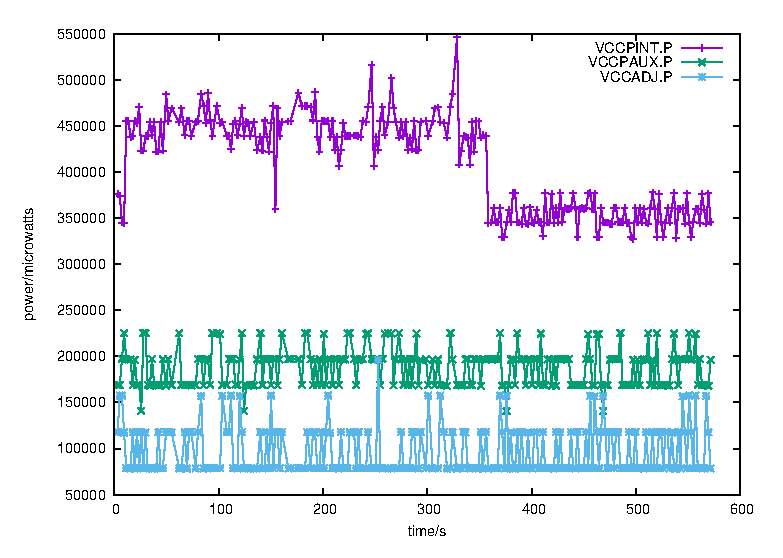
\includegraphics[width=\textwidth]{data/fig/vtr:pow:667.eps}
      \caption{Power usage of VTR at 667MHz}
      \label{fig:vtr:pow:667}
    \end{figure}
    \begin{figure}[p]
      \includegraphics[width=\textwidth]{data/fig/vtr:pow:333.eps}
      \caption{Power usage of VTR at 333MHz}
      \label{fig:vtr:pow:333}
    \end{figure}
    There is a clear uptick in VCCPINT usage after the first 4 samples, which is when the test is started. There is a large deviation in VCCPINT draw over the course of the benchmark at 667MHz, but a signifcantly reduced deviation when run at 333MHz - which I propose is due to the fewer stalls of the processor on memory accesses. On the other hand, VCCADJ's power usage at 333MHz is consistently higher, whilst at 667MHz, it peaks briefly but then returns to baseline for a much longer time - a behaviour I suggest follows on from it being able to complete trannsfers in a shorter time at the higher clock rate, enabling it to return the memory bus to idle sooner.

  \subsection{Memory}
    Figures \ref{fig:vtr:mem:667} and \ref{fig:vtr:mem:333} show system memory usage for active pages, anonymous pages and the total committed address space during the running of the VTR tests.
    \begin{figure}[p]
      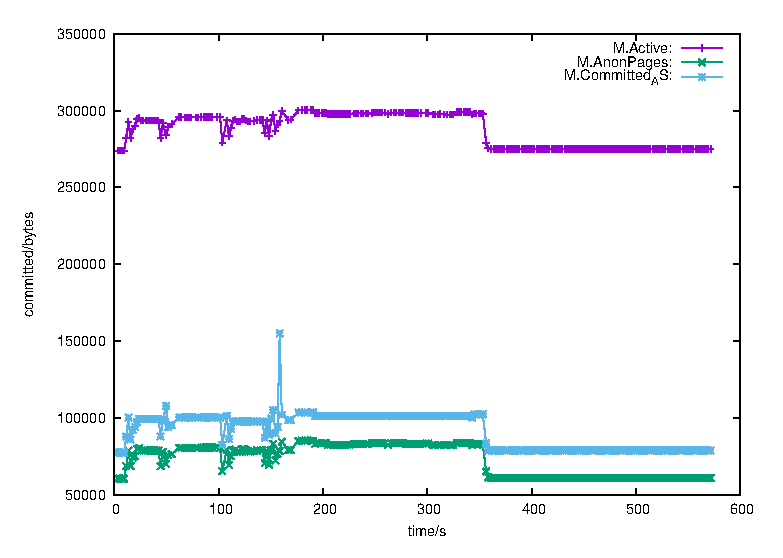
\includegraphics[width=\textwidth]{data/fig/vtr:mem:667.eps}
      \caption{Memory usage of VTR at 667MHz}
      \label{fig:vtr:mem:667}
    \end{figure}
    \begin{figure}[p]
      \includegraphics[width=\textwidth]{data/fig/vtr:mem:333.eps}
      \caption{Memory usage of VTR at 333MHz}
      \label{fig:vtr:mem:333}
    \end{figure}
    These show the allocated of anonymous pages for VTR (and its assosciated tools) to run in. The profiles are pretty similar during both sets of tests, due to changing the speed having little effect on the amount of memory needed. The major spikes in committed address space correspond directly to sudden decreases in the number of active pages - possibly an effect of the deallocations having occurred but the address space not being marked as uncommitted until after the next set of allocations has occurred.

\section{x264}
  \subsection{Runtime}
    Table \ref{tab:x264:rt} shows the runtime for the various PS clock speeds.
    \begin{table}[bp]
      \centering
      \begin{tabular}{l | l}
        Speed/MHz & Runtime/s \\
        \hline
        333 & 122 \\
        667 & 62 \\
      \end{tabular}
      \caption{Runtime vs Speed of PS for x264 encoding}
      \label{tab:x264:rt}
    \end{table}
    Unlike the VTR benchmarks, the runtime is unaffected by the speed of the processor core, despite making heaving usage of NEON optimizations, the limitation is clearly elsewhere\ldots

  \subsection{Power}
    Figures \ref{fig:x264:pow:667} and \ref{fig:x264:pow:333} shows the 'power' as reported by the PMIC for the VCCPx rails and VCCADJ rail.
    \begin{figure}[p]
      \includegraphics[width=\textwidth]{data/fig/x264:pow:667.eps}
      \caption{Power usage of x264 at 667MHz}
      \label{fig:x264:pow:667}
    \end{figure}
    \begin{figure}[p]
      \includegraphics[width=\textwidth]{data/fig/x264:pow:333.eps}
      \caption{Power usage of x264 at 333MHz}
      \label{fig:x264:pow:333}
    \end{figure}
    At 667MHz, there is an increase of 250mW on VCCPINT for the ~62 seconds, but for 333MHz, there is an increase of only 120mW for the 122 seconds, indicating that running at 333MHz consumes less power in total for the same task.


  \subsection{Memory}

\end{document}
